\documentclass[12pt,a4paper]{article}

\usepackage{a4wide}
\usepackage{graphicx}
\usepackage{amsmath}
\usepackage{ae,aecompl}
\usepackage{amsthm}

%\pagestyle{empty}
\setlength{\parindent}{0pt}
\renewcommand{\labelenumi}{\alph{enumi})}
\renewcommand{\labelenumii}{\roman{enumii})}

% Neutrino oscillation channels
\newcommand{\ee}{\ensuremath{\nu_e \rightarrow \nu_e}}
\newcommand{\emu}{\ensuremath{\nu_e \rightarrow \nu_\mu}}
\newcommand{\etau}{\ensuremath{\nu_e \rightarrow \nu_\tau}}
\newcommand{\mue}{\ensuremath{\nu_\mu \rightarrow \nu_e}}
\newcommand{\mumu}{\ensuremath{\nu_\mu \rightarrow \nu_\mu}}
\newcommand{\mutau}{\ensuremath{\nu_\mu \rightarrow \nu_\tau}}
\newcommand{\taue}{\ensuremath{\nu_\tau \rightarrow \nu_e}}
\newcommand{\taumu}{\ensuremath{\nu_\tau \rightarrow \nu_\mu}}
\newcommand{\tautau}{\ensuremath{\nu_\tau \rightarrow \nu_\tau}}

% Neutrino oscillation parameters
\newcommand{\sthsol}{\ensuremath{\sin^2 2\theta_{12}}}     % Mixing angles
\newcommand{\sthchooz}{\ensuremath{\sin^2 2\theta_{13}}}
\newcommand{\sthatm}{\ensuremath{\sin^2 2\theta_{23}}}
\newcommand{\sthtf}{\ensuremath{\sin^2 2\theta_{2f}}}
\newcommand{\ldm}{\ensuremath{{\Delta m_{31}^2}}}          % Mass squared differences
\newcommand{\sdm}{\ensuremath{{\Delta m_{21}^2}}}

% Important neutrino experiments
\newcommand{\TtoK}{{\sffamily T2K}}

% Miscellaneous commands
\newcommand{\aufg}[2]{\vspace{4mm}{\bf\underline{Problem #1:} {#2}} \vspace{3mm}}

% Environment for API reference entries
\newtheoremstyle{dotless}{}{}{\itshape}{}{\bfseries}{}{0cm}{}
\theoremstyle{dotless}
\newtheorem*{function}{}

\begin{document}
\vspace*{-3cm}
\begin{center}
{\large\bf GLoBES Tutorial: Advanced Usage of AEDL}\\ [0.3cm]
GLoBES workshop in Heidelberg, Germany, January 24-26, 2007
\end{center}
\vspace*{2mm}

Mark Rolinec \hfill 25.01.07

\bigskip
\hrule
\vspace*{4mm}

{\small
This tutorial will adress basic and advanced features of the {\bf A}bstract 
{\bf E}xperiment {\bf D}efinition {\bf L}anguage AEDL. The syntax of AEDL is
comprehensive and thus allows to define all different kinds of neutrino 
oscillation experiments with different neutrino sources and different detector
technologies. Within this tutorial we will define a toy experiment by using 
the most important features of AEDL and get familiar with the AEDL syntax.
Then we will modifiy the experiment description going from basic usage of AEDL
to more advanced features. After that we will explore some of the pre-defined
AEDL files that come with GLoBES 3.0 and analyze advanced features in their AEDL
description. \\

The toy experiment for this tutorial is absolutely fictious, although the attributes 
of the detector follow roughly the response of a huge Water Cerenkov detector.
However, all efficiencies and migration matrices are coming from a fake 
Monte Carlo simulation and do {\bf not} exactly correspond to the true 
attributes of a Water Cerenkov detector. So, all files prepared for this tutorial 
do {\bf not} correspond to a real detector response and all files are just to 
be used for this tutorial.  
}


% ----------------------------------------------------------------------------
\section*{Part 1: AEDL implementation of a toy experiment}
% ----------------------------------------------------------------------------

Suppose you work for a collaboration that plans to build a long baseline 
neutrino oscillation experiment with a flavor-pure neutrino beam, that consists 
either of $\nu_e$ or $\bar{\nu}_e$. It is planned to build a huge {\em modified} 
Water Cerenkov detector. Now, you want to analyze the future potential of the 
experiment and maybe try to optimize some of the attributes. Your decision is to
do the analysis with GLoBES. So, first you have to build the experiment description
in AEDL,~{\it i.e.} write the corresponding {\tt glb}-file. One of your colleagues
sends the results from a Monte Carlo analysis. 
\begin{figure}[h!]
  \begin{center}
    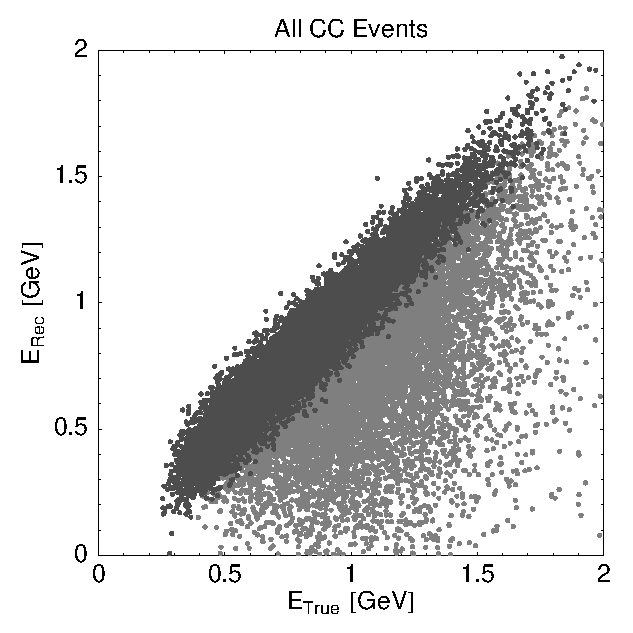
\includegraphics[width=0.36\textwidth]{CCevents.eps} \hspace{0.5cm}
    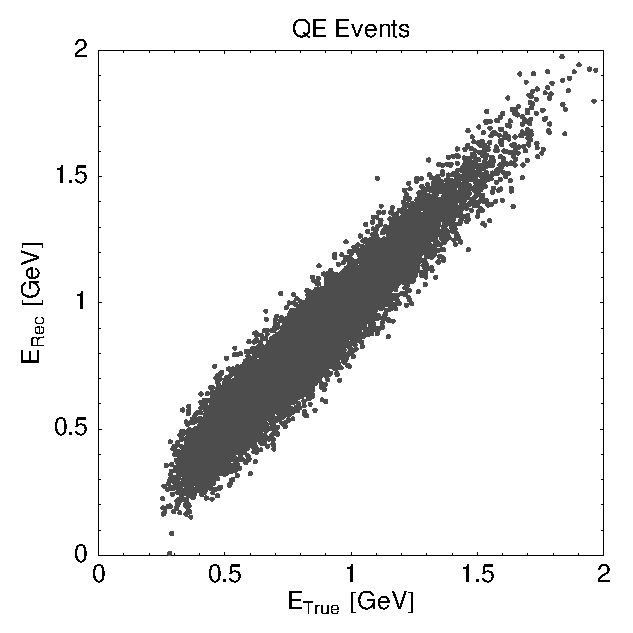
\includegraphics[width=0.36\textwidth]{QEevents.eps}
  \end{center}
  \vspace{-0.7 cm}
  \caption{\small The sample of 20000 charged current $\nu_\mu$ events on the left hand side. The
  quasi-elastic sample is shown in dark grey while the inelastic part of the sample is
  shown in bright grey. The quasi-elastic part of the sample alone is plotted at the right-hand
  side. It can be seen that this sample allows to recontruct the true neutrino energy at a
  certain level, while this is not possible for the inelastic part of the sample.}
  \label{fig:mccc}
\end{figure}

It is also important to implement the background from single pion production in 
neutral current events. Therefore, the colleague sends the Monte Carlo sample of NC events.

\begin{figure}[h!]
  \begin{center}
    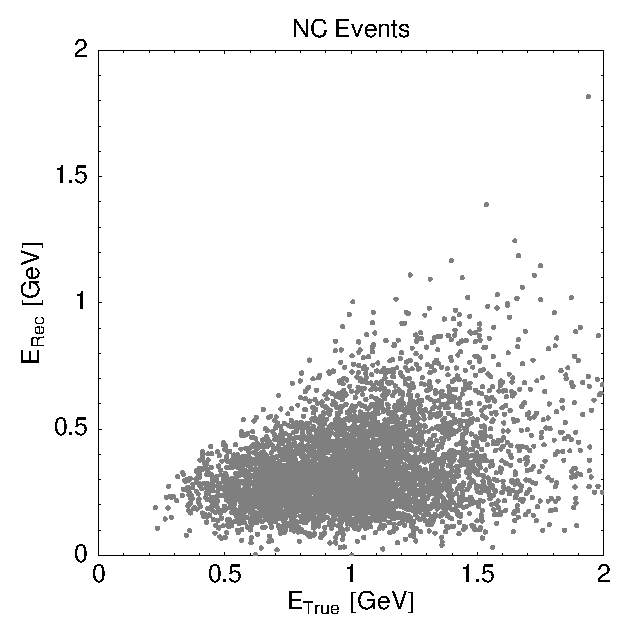
\includegraphics[width=0.45\textwidth]{NCevents.eps} 
  \end{center}
  \vspace{-0.7 cm}
  \caption{\small The sample of 5000 neutral current events. It can be seen that the
  reconstructed energy is systematically smaller than the true neutrino energy since
  there is missing energy due to the undetected neutrino in the NC event.}
  \label{fig:mcnc}
\end{figure}

The colleague also sends the energy dependent signal efficiencies of the charged
current $\nu_\mu$/$\bar{\nu}_\mu$ events from the Monte Carlo simulations. These 
include the Cerenkov threshold for muons. They are given for 18 bins of 
$\mathrm{\Delta E=0.1\, GeV}$ between 0.2~GeV and 2.0~GeV (The list of these energy dependent
efficiecies is given in the files {\tt NUMUeff.dat} and {\tt NUMUBAReff.dat}).
Furthermore, he tells you that the rejection factor for the NC events should be $10^-3$.
This is all the information needed to reconstruct smearing matrices out of the data
that can be used to describe the experiment in an AEDL file.

\aufg{1}{Warm-Up}

The smearing matrices are provided in the files {\tt CCmigration.dat}, {\tt CCBARmigration.dat},
and {\tt NCmigration.dat}. They are already given in the right syntax, so that they can be
implemented into an AEDL file. However, try to qualitatively understand, how these matrices 
can be reconstructed from the data given above. If you are not familiar with the usage of
manually defined smearing matrices, please consult the GLoBES manual on pages 101-102.

\aufg{2}{Finding the Normalization}

Another colleague of yours provides you with the data of the neutrino beam flux. This is given
in the files {\tt TOYplus.dat} ($\nu_e$) and {\tt TOYminus.dat} ($\bar{\nu}_e$), already provided 
in the right syntax for GLoBES. The implementation of neutrino fluxes from a data file is described in the 
GLoBES manual on pages 89-90.

\begin{figure}[h!]
  \begin{center}
    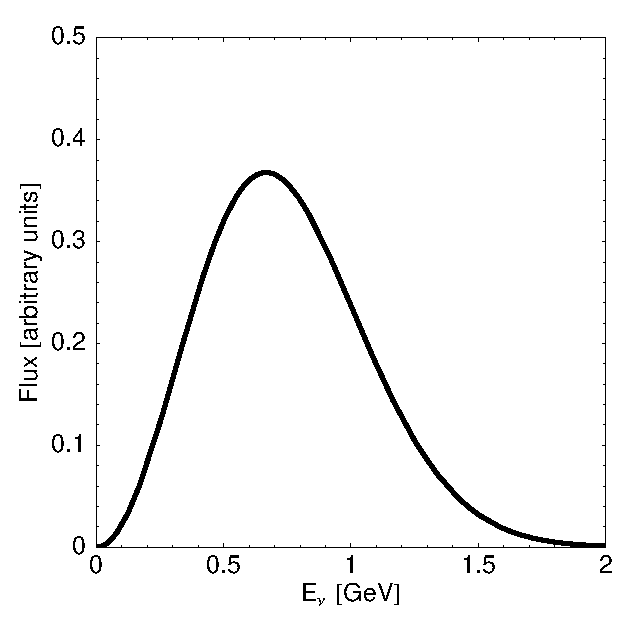
\includegraphics[width=0.45\textwidth]{FLUX.eps} 
  \end{center}
  \vspace{-0.7 cm}
  \caption{\small The neutrino flux of the toy experiment as a function of the neutrino energy.
  The flux is given in arbitrary units so the right normalization has to be found.}
  \label{fig:flux}
\end{figure}

Unfortunately, your colleague does not know the units of the flux data anymore, but he 
tells you that his Monte Carlo simulation showed that in case of no oscillations 
he would get at total number of 13503.5 $\nu_e$ charged current events and 
4612.18 $\bar{\nu}_e$ charged current events per kt and year at the planned baseline 
of L~=~350~km. He tells you that they estimated a new average matter density along the
baseline of $\rho=2.95\,g/cm^3$. \\

Start from the draft file {\tt TOYdraft.glb} and build an AEDL file that
uses the flux files and allows to calculate the unoscillated $\nu_e/\bar{\nu}_e$ CC events per kt and
year. Use 18 bins from 0.2~GeV to 2~GeV (necessary, since the migration matrices are given for this binning). 
Calculate the event rates with the
command {\tt globes} from the {\tt /source} directory. Within {\tt TOYdraft.glb}  
you can find some hints where the corresponding AEDL features are documented in the GLoBES
manual.

\aufg{3}{Describing the Experiment}

Now, that we have found the right normalization, we can describe the toy experiment. The detector will
be located at the baseline of L~=~350~km and have a fiducial mass of 500~kt. The experiment
will measure $\nu_\mu$-appearance and $\bar{\nu}_\mu$-appearance. For collecting comparable
amount of data in both channels, it is planned to have split mode of operation,~{\it i.e.}
2 years in $\nu_e$ mode and 6 years in $\bar{\nu}_e$ mode. It is assumed that the overall
normalization uncertainty of the signal events will be 2.5\% and 20\% on the background events. \\

Build up an AEDL file that decribes the experiment and makes use of the migration matrices.
Note, that the migration matrices are for CC and NC events. \\

Check your AEDL file with the {\tt globes} command for the following oscillation parameters:
\begin{eqnarray}
\sin^2\theta_{12} & = & 0.3 \nonumber \\
\sin^22\theta_{13} & = & 0.1  \nonumber \\
\sin^22\theta_{23} & = & 1  \nonumber \\
\delta_{CP} & = & \pi/2  \nonumber \\
\Delta^2_{21} & = & 7.9\cdot 10^{-5}\, eV^2  \nonumber \\
\Delta^2_{31} & = & 2.6\cdot 10^{-3}\, eV^2  
\end{eqnarray}
This can be done with the command 
\begin{center}
{\tt ./globes -p'0.5796,0.1609,0.7854,1.5708,7.9e-5,2.6e-3' NAME.glb}
\end{center}

This is what you should be obtained (signal and background event numbers):\\

{\tt 
\hspace*{2cm} --------- \#NU\_MU\_Appearance ---------\\
\hspace*{2cm}               233787 ||       233787\\
\hspace*{2cm}              4640.85 ||      4640.85\\
\hspace*{2cm} \\
\hspace*{2cm} \\
\hspace*{2cm} --------- \#NU\_MU\_BAR\_Appearance ---------\\
\hspace*{2cm}               173047 ||       173047\\
\hspace*{2cm}              4911.57 ||      4911.57\\
}

The binned event rates can be calculated with the command {\tt ./globes -s NAME.glb}. The screen output that should be
derived is given in the appendix.  \\

Furthermore, the program {\tt th13delta.c} and the script {\tt th13delta.gnuplot} can be used
to produce a contour plot of the best fit solution in the $\sin^22\theta_{13}$-$\delta_{CP}$-plane (there are still degenerate solutions left 
in different locations of the parameter space,~{\it i.e.} the intrinsic and the
sign-degeneracy). Do not forget to enter the Name of your AEDL file into {\tt th13delta.c}.
Note, that another AEDL file is loaded within {\tt th13delta.c}, {\tt T2K\_disappearance\_only.glb}. This is due to
the fact, that the leading atmospheric parameters cannot be measured at the toy experiment. This can spoil the
results through parameter correlations. Thus, the simulated disappearance data from T2K is included. The T2K appearance
data is missing, so that information on $\sin^22\theta_{13}$ and $\delta_{CP}$ can only be derived from the toy
experiment data. The effect can be seen in Fig.~\ref{fig:withoutT2K} in the appendix. 


\aufg{4}{Experiment Description without Smearing Matrices}

One of your colleagues tells you, that the energy reconstruction of the quasi-elastic
events follows a gaussian energy resolution function with a width of $\sigma=0.085\, GeV$.
The smearing is due to Fermi Motion and so in his analysis he found that this width is
independent of the neutrino energy over the whole energy window up to 2 GeV. \\

Modify the AEDL file in such a way that no migration matrices are used anymore. You will need
the efficiency and background rejection data from the files {\tt NUMUeff.dat}, {\tt
NUMUBAReff.dat}, {\tt NC\_bckg\_rej.dat}, and {\tt NCBAR\_bckg\_rej.dat}. Make use of the
GLoBES built-in energy resolution function. Then, compare the event rates and the best-fit
solution you get from this file with the file from the former problem. You should approximately
end up with this output:\\

{\tt  
\hspace*{2cm} --------- \#NU\_MU\_Appearance --------- \\
\hspace*{2cm}               222833 ||       222833 \\
\hspace*{2cm}               4640.5 ||       4640.5 \\
\hspace*{2cm}  \\
\hspace*{2cm}  \\
\hspace*{2cm} --------- \#NU\_MU\_BAR\_Appearance --------- \\
\hspace*{2cm}               171644 ||       171644 \\
\hspace*{2cm}              4911.57 ||      4911.57 \\
}

The binned event rates again can be derived with the command {\tt ./globes -s NAME.glb}. The screen output 
that should be obtained is given in the appendix. \\

Now we can compare the best-fit solution from the file with migration matrices and the 
file without migration matrices:

\begin{figure}[h!]
  \begin{center}
    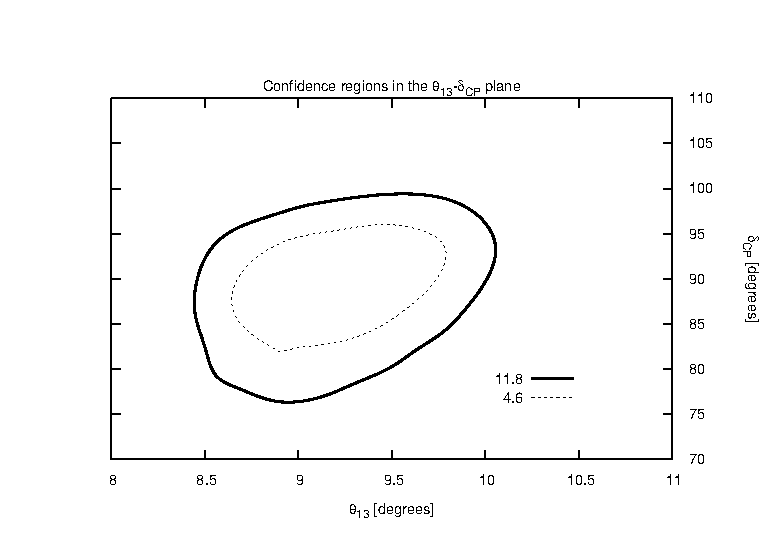
\includegraphics[width=0.48\textwidth]{WithMatrices.eps}   
    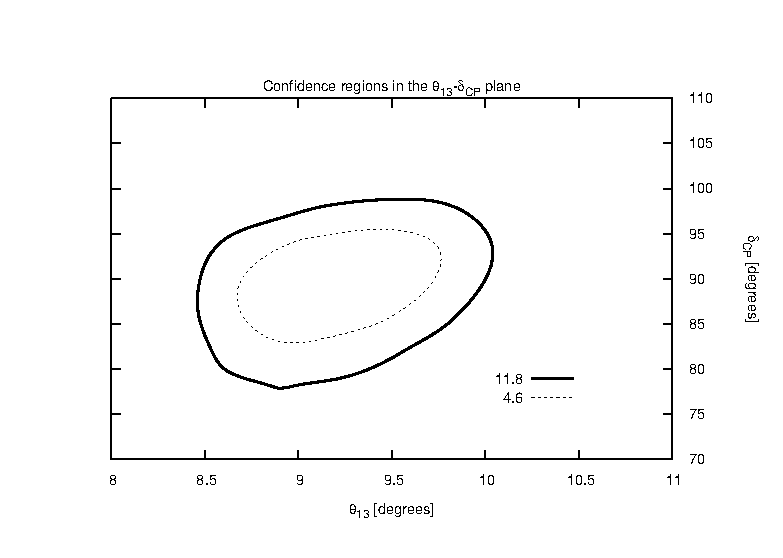
\includegraphics[width=0.48\textwidth]{WithoutMatrices.eps} 
  \end{center}
  \vspace{-0.7 cm}
  \caption{\small Left-Hand Side: The allowed best-fit solution obtained with {\tt th13delta.c}
  and the toy experiment description using manually defined migration matrices. Right-Hand Side: 
  The allowed best-fit solution obtained with {\tt th13delta.c}
  and the toy experiment description using the GLoBES internal energy resolution function.}
  \label{fig:Comp}
\end{figure}


\aufg{5}{List Interpolation in AEDL}

The description of the experiment without migration matrices has one big advantage
in comparison to the description with migration matrices. Suppose, one of your colleagues
wants to compare your analyisis with your analysis. Unfortunately, he uses 16 bins instead of
18 and asks you to do the same. One could either do the same procedure again and prepare
completely new migration matrices, this time $16\times16$. But, this would of course be very
time consuming. Or one can use the former description and introduce the efficiencies 
by applying the AEDL feature of list interpolation as described in the GLoBES manual 
on pages 84-85. The result should of course look extremely similar.

\begin{figure}[h!]
  \begin{center}
    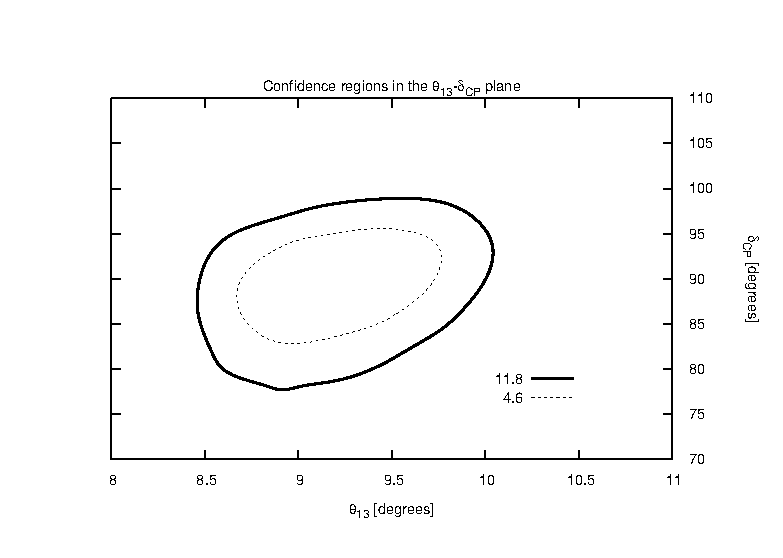
\includegraphics[width=0.5\textwidth]{Bins.eps}   
      \end{center}
  \vspace{-0.7 cm}
  \caption{\small The allowed best-fit solution obtained with {\tt th13delta.c}
  and the toy experiment description using the GLoBES internal energy resolution function.
  and 16 bins with efficiencies obtained with the AEDL list interpolation feature.}
  \label{fig:Bins}
\end{figure}


\aufg{6}{Usage of Total Rates}

The former files only make use of the quasi-elastic event sample, since there energy
reconstruction is possible to a certain level. However, this reduces the statistics of the
experiment, because all inelastic events are omitted.\\

The CC current events can be included to the file and the systematics function
{\tt chiTotalRatesTilt} within the corresponding rule can be used to only count 
total rates. The spectral information still comes from the QE events. However, now double
counting of events has to be avoided. Therefore the QE events have to be taken into account
with a free normalization. The explanations about the needed systematics functions can be found
in the GLoBES manual on pages 105-106. You can also check the {\tt T2K.glb} file. There, this
description is already implemented. Please discuss the systematics function, that has to be
used for the QE events in case of no treatment of systematics.\\

In the end you should end up at:\\

{\tt
\hspace*{2cm} --------- \#NU\_MU\_Appearance\_QE ---------\\
\hspace*{2cm}               222706 ||       222706\\
\hspace*{2cm}              4840.44 ||      4840.44\\
\hspace*{2cm} \\
\hspace*{2cm} \\
\hspace*{2cm} --------- \#NU\_MU\_BAR\_Appearance\_QE ---------\\
\hspace*{2cm}               171630 ||       171630\\
\hspace*{2cm}              5169.42 ||      5169.42\\
\hspace*{2cm} \\
\hspace*{2cm} \\
\hspace*{2cm} --------- \#NU\_MU\_Appearance\_CC ---------\\
\hspace*{2cm}               379842 ||       379842\\
\hspace*{2cm}              4840.44 ||      4840.44\\
\hspace*{2cm} \\
\hspace*{2cm} \\
\hspace*{2cm} --------- \#NU\_MU\_BAR\_Appearance\_CC ---------\\
\hspace*{2cm}               265792 ||       265792\\
\hspace*{2cm}              5169.42 ||      5169.42\\
}

\begin{figure}[h!]
  \begin{center}
    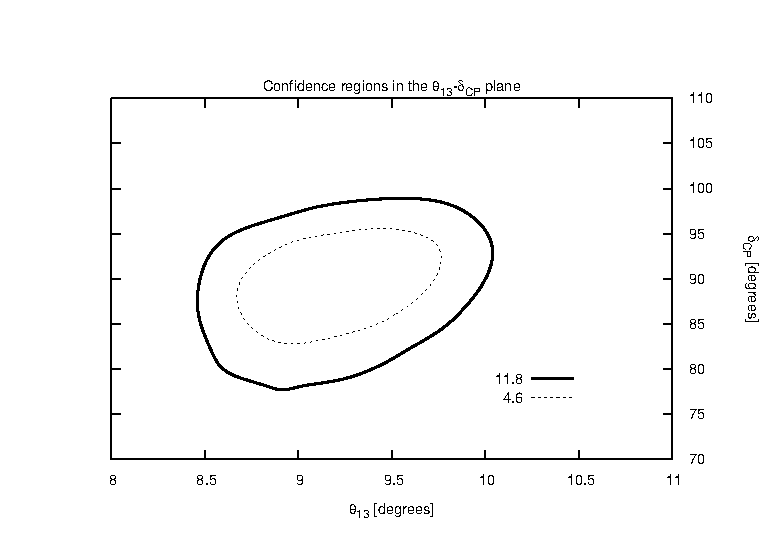
\includegraphics[width=0.5\textwidth]{CCtotal.eps}   
      \end{center}
  \vspace{-0.7 cm}
  \caption{\small The allowed best-fit solution obtained with {\tt th13delta.c}
  and the toy experiment description using the GLoBES internal energy resolution function.
  Here, the total rates data from all CC events and the spectral data from the QE sample
  with a free normalization is used within the analysis.}
  \label{fig:total}
\end{figure}

The difference to the former simulations is not very large. This is due to the fact that
the true value of $\sin^22\theta_{13}$ is chosen quite large. For smaller $\sin^22\theta_{13}$
the effect becomes more important, since overall statistics decrease and the additional statistics
improves the results in a more dramatic way.

% ----------------------------------------------------------------------------
\section*{Part 2: Features of the Pre-Defined AEDL Experiments}
% ----------------------------------------------------------------------------

Now, we can have a look at the pre-defined AEDL experiments. The problems of
Part 1 have made us familiar with the syntax of AEDL. One of the most important
AEDL features used in the variable AEDL files is the usage of AEDL variables.
For instance the the file {\tt data/NuFact/Variable/NFvar.glb} is defined with free
parameters. First, we can have a look at the implementation of the neutrino factory
flux. In contary to the toy experiment, the fluxes are not loaded from a data file, but
derived from the built-in flux feature of GLoBES. The parent energy and the baseline of the
experiment is kept free and can be specified by usage of the AEDL variables {\tt emax} and
{\tt BASELINE}.\\

Copy the file {\tt source/globes} to the directory with the {\tt NFvar.glb} file and try the
command:
\begin{center}
{\tt ./globes -DBASELINE=3000 -Demax=50 NFvar.glb}
\end{center}

Furthermore, the file {\tt NFvar.glb} makes use of the AEDL feature to allow variable
binwidths. The binwiths are chosen such that the bins at smaller energies are more narrow than
for larger energies. This is done, because the energy resolution is proportional to the
neutrino energy and a better resolution is obtained at smaller energies, which requires
smaller binning. However, the absolute position of the bins depends on {\tt emax} so that
it is not possible to give fixed efficiency lists. Here, the new interpolation feature
of GLoBES is necessary.\\


The implementation of a built-in beta beam flux can be explored
in the variable beta beam file {\tt data/BetaBeam/BB\_WC/BBvar\_WC.glb}. Here, also AEDL variables have been
introduced to allow an analysis of beta beams by modifying the $\gamma$ factor and the
baseline. Since for this experiment migration matrices cannot be used to maintain the
variability, the same technique as in Problem 6 is used. 

\newpage
\begin{appendix}
\section{Effect of T2K Disappearance Data}

\begin{figure}[h!]
  \begin{center}
    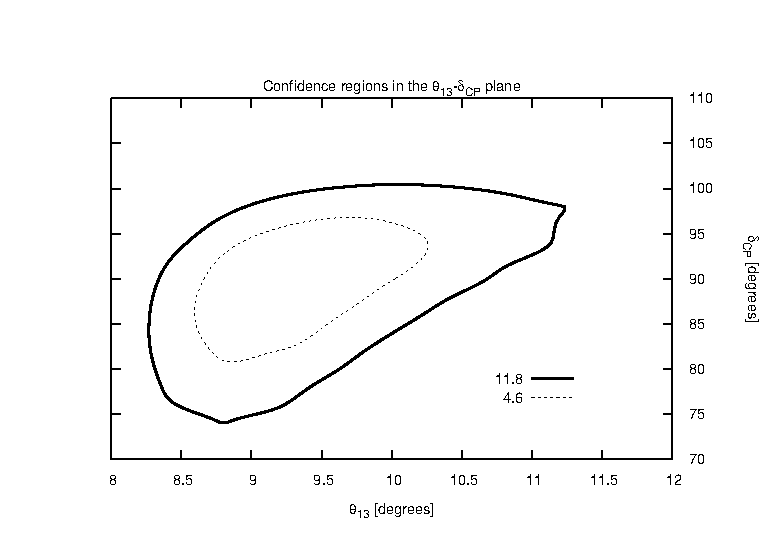
\includegraphics[width=0.5\textwidth]{WITHOUT_T2K.eps}   
      \end{center}
  \vspace{-0.7 cm}
  \caption{\small The allowed best-fit solution obtained with {\tt th13delta.c}
  and the toy experiment description using migration matrices. The disappearance data from
  T2K is {\bf not} used here.}
  \label{fig:withoutT2K}
\end{figure}

\section{Spectral Event Rates}

\footnotesize \tt

\begin {center}
\begin{tabular}{lcl}

{\large Migration Matrices} && {\large Energy Resolution Function} \\ \hline && \\ 
--------- \#NU\_MU\_Appearance ---------&&--------- \#NU\_MU\_Appearance ---------\\
&&\\
  0.25       3235.32&&  0.25       872.803\\
  0.35        8516.4&&  0.35       4161.83\\
  0.45       18670.5&&  0.45       13747.8\\
  0.55       30845.9&&  0.55       27084.3\\
  0.65         37326&&  0.65       35648.9\\
  0.75       36255.2&&  0.75       36404.7\\
  0.85       30234.2&&  0.85       32152.6\\
  0.95       23895.9&&  0.95       25359.3\\
  1.05         17472&&  1.05       18206.2\\
  1.15       11164.9&&  1.15       12112.7\\
  1.25       7213.56&&  1.25       7574.92\\
  1.35       4387.87&&  1.35       4499.13\\
  1.45        2290.2&&  1.45       2501.03\\
  1.55       1175.12&&  1.55        1317.7\\
  1.65       573.792&&  1.65       668.669\\
  1.75       287.307&&  1.75       317.866\\
  1.85       158.537&&  1.85       143.546\\
  1.95        83.849&&  1.95       58.5287\\
----------------------&&----------------------\\
Total:        233787&&Total:        222833\\
&&\\
  0.25       1899.59&&  0.25       1899.63\\
  0.35       1379.43&&  0.35       1379.05\\
  0.45       707.324&&  0.45       707.319\\
  0.55       347.565&&  0.55       347.565\\
  0.65       161.629&&  0.65       161.629\\
  0.75       75.6928&&  0.75       75.6928\\
  0.85       41.3034&&  0.85       41.3034\\
  0.95       17.3519&&  0.95       17.3519\\
  1.05        6.3722&&  1.05        6.3722\\
  1.15       3.16321&&  1.15       3.16321\\
  1.25       0.53009&&  1.25       0.53009\\
  1.35      0.598437&&  1.35      0.598437\\
  1.45             0&&  1.45   0.000143515\\
  1.55             0&&  1.55   8.79703e-05\\
  1.65             0&&  1.65   5.08887e-05\\
  1.75             0&&  1.75   2.78955e-05\\
  1.85      0.298004&&  1.85      0.298002\\
  1.95             0&&  1.95    7.1521e-06\\
----------------------&&----------------------\\
Total:       4640.85&&Total:        4640.5\\
\end{tabular}
\end{center}

\newpage

\begin {center}
\begin{tabular}{lcl}

{\large Migration Matrices} && {\large Energy Resolution Function} \\ \hline && \\ 
--------- \#NU\_MU\_BAR\_Appearance ---------&&--------- \#NU\_MU\_BAR\_Appearance ---------\\
&&\\
  0.25       1110.29&&  0.25       430.704\\
  0.35        3257.3&&  0.35       1595.73\\
  0.45       9112.41&&  0.45       5209.66\\
  0.55       15748.8&&  0.55         12256\\
  0.65         19876&&  0.65       20000.1\\
  0.75       24939.8&&  0.75       25053.5\\
  0.85       24582.1&&  0.85         25888\\
  0.95       20723.2&&  0.95       23282.3\\
  1.05       17965.5&&  1.05       19168.5\\
  1.15       13890.8&&  1.15       14457.6\\
  1.25       8845.95&&  1.25       10004.5\\
  1.35       5449.44&&  1.35       6349.17\\
  1.45       3585.94&&  1.45       3729.31\\
  1.55       1870.27&&  1.55       2099.19\\
  1.65       1027.29&&  1.65       1137.16\\
  1.75       559.153&&  1.75       582.734\\
  1.85       330.635&&  1.85        280.22\\
  1.95       172.192&&  1.95       119.721\\
----------------------&&----------------------\\
Total:        173047&&Total:        171644\\
&&\\
  0.25       1882.64&&  0.25       1882.64\\
  0.35        1436.5&&  0.35       1436.51\\
  0.45       790.672&&  0.45       790.666\\
  0.55       412.492&&  0.55       412.492\\
  0.65        201.96&&  0.65        201.96\\
  0.75       95.6634&&  0.75       95.6634\\
  0.85       53.6873&&  0.85       53.6873\\
  0.95       22.8585&&  0.95       22.8585\\
  1.05       8.63062&&  1.05       8.63062\\
  1.15       4.40415&&  1.15       4.40415\\
  1.25      0.765549&&  1.25      0.765549\\
  1.35      0.843628&&  1.35      0.843628\\
  1.45             0&&  1.45    0.00019704\\
  1.55             0&&  1.55   0.000124013\\
  1.65             0&&  1.65   7.34927e-05\\
  1.75             0&&  1.75   4.11518e-05\\
  1.85      0.455293&&  1.85      0.455293\\
  1.95             0&&  1.95    1.0927e-05\\
----------------------&&----------------------\\
Total:       4911.57&&Total:       4911.57

\end{tabular}
\end{center}

\end{appendix}








\end{document}


